\section{Result and interpretation}
\label{sec:result}

For each \zd signal, an independent cut-and-count analysis is performed on a \mass{Z2} window and 
a limit on cross section for each \mass{\zd} is reported. The center of the window is taken to be 
the assumed \mass{\zd} value and the widths for each \mass{\zd} value are chosen as described in
Section~\ref{sec:masswindow}. Limits on cross sections are calculated with the asymptotic formula for the 
$\mathrm{CL_s}$ test statistic, as described in~\cite{CMS-NOTE-2011-005}. Cross sections of 
\zd signal for each mass value are taken from~\cite{Curtin:2014cca}, as described in Section~\ref{sec:datamc}.

The likelihood $\mathcal{L}$, as a product of likelihood functions
for 2016, 2017 and 2018 event samples, is defined in Equation \ref{eq:LHC-Likelihood}.
\begin{equation}
	 \label{eq:LHC-Likelihood}
	  \mathcal{L}(\mathrm{data} \, | \, \mu, \theta ) = \mathrm{Poisson} \left( \, N| \, \mu \cdot s( \theta ) + b( \theta ) \, \right) \cdot p(\tilde{\theta} \, | \, \theta ) \, .
\end{equation}

where $N$ is the number of observed events, $s$ is the expected
signal, and $b$ is the expected background rate in the sample, 
The parameter $\mu =\sigma/\sigma_{theo}$, the ratio of the
measured to the predicted cross section, is the signal-strength modifier and
$\theta$ represents the full range of nuisance parameters, where $\tilde
\theta$ is the best estimate of the nuisance prior to the data analysis.
$\mathrm{Poisson}(N|\mu \cdot s(\theta) + b(\theta)))$ stands
for the Poisson probability to observe $N$
events given the expected event rate $\mu \cdot s(\theta) +
b(\theta)$. The probability $p(\tilde \theta | \theta )$ encode
information on the systematic uncertainties. The maximum likelihood estimates of $\mu$ and $\theta$ are
denoted as $\hat \mu$ and $\hat \theta$, whereas $\hat \theta_{\mu}$
denotes the conditional maximum likelihood estimate of all nuisance
parameters with a fixed signal strength modifier $\mu$.

With the upper limit of signal cross section at each \mass{\zd} value, 
the  95\% confidence level (CL) upper limit on the kinematic mixing parameter and 
$Br(H \rightarrow Z \zd)$ are calculated and reported in Figure~\ref{fig:limit}. 

\begin{figure}[!htb]
\vspace*{0.3cm}
\centering
{ 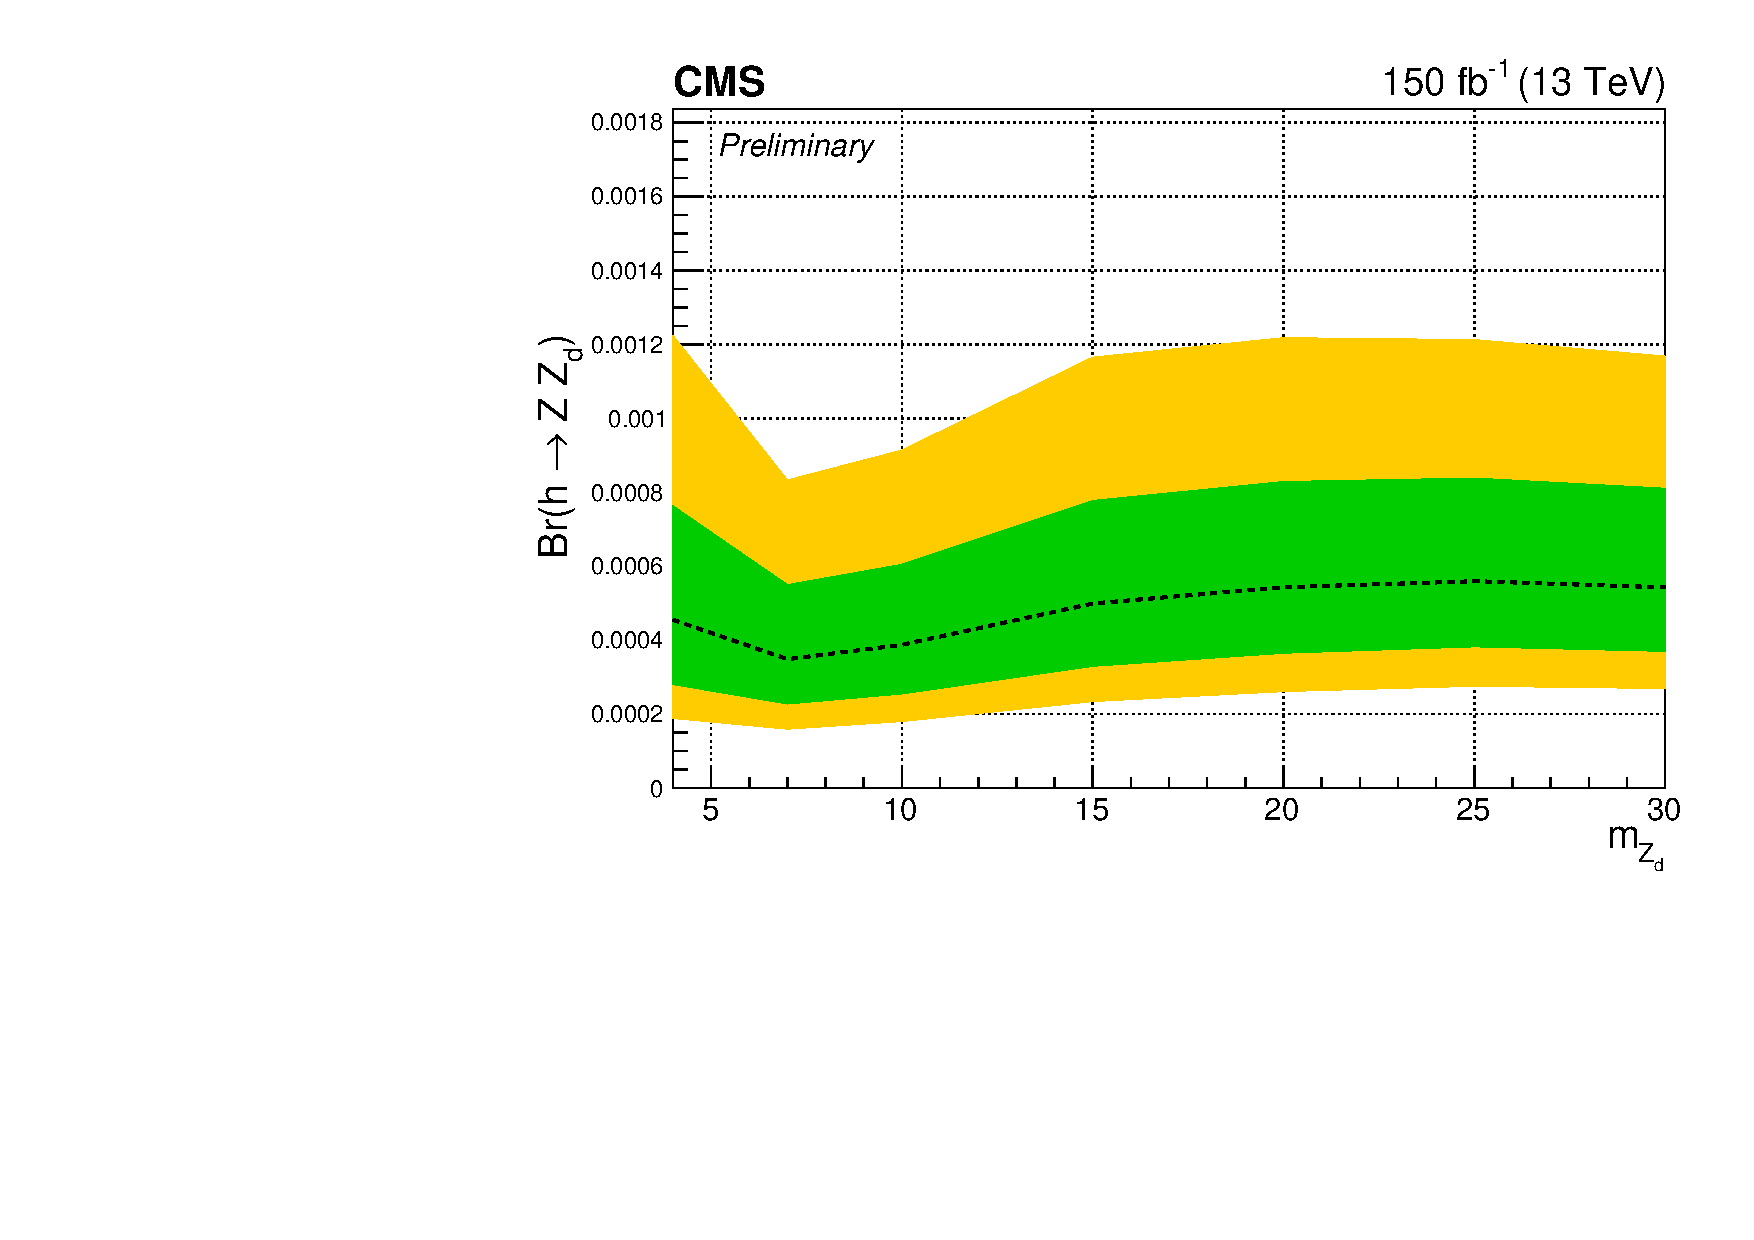
\includegraphics[width=0.48\textwidth]{Figures/Results/Limit/ExpLimit_BrHZZd}}
{ 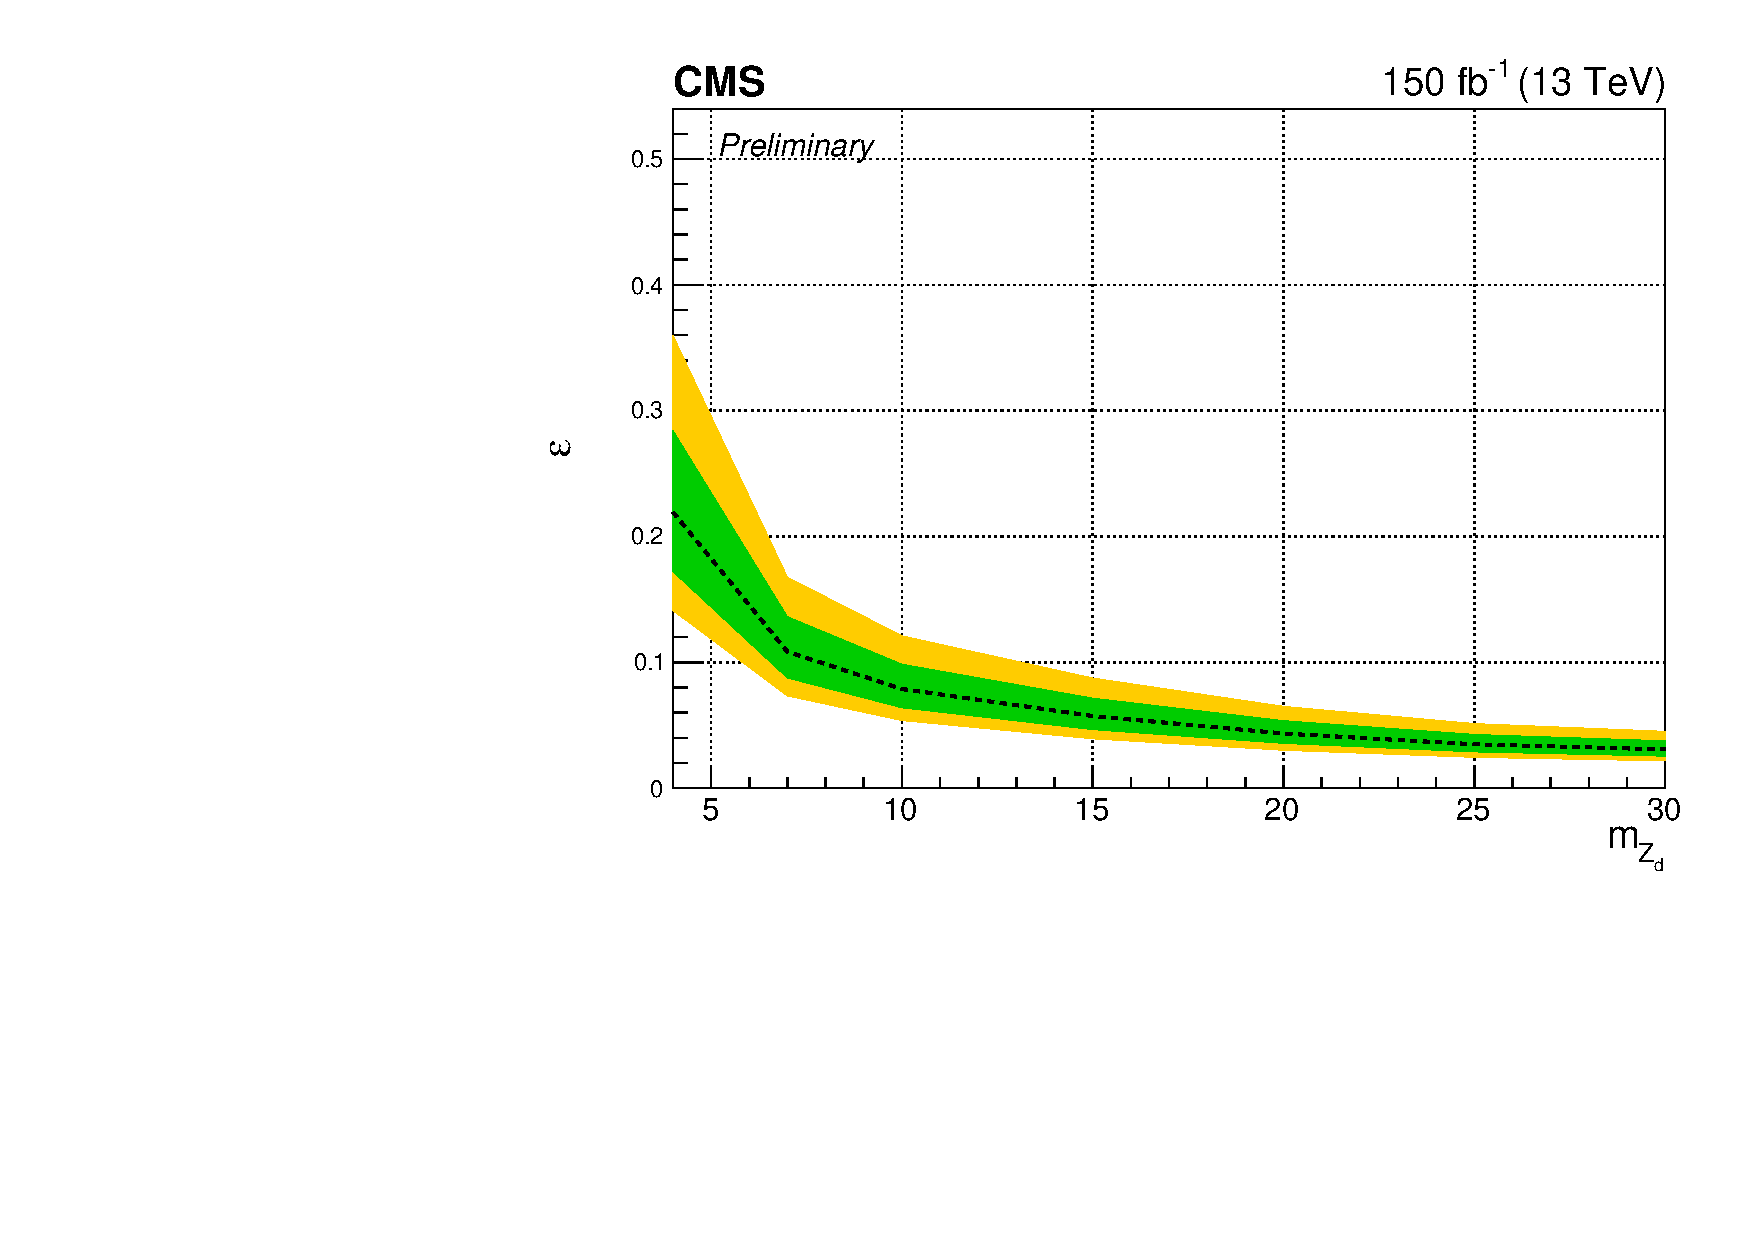
\includegraphics[width=0.48\textwidth]{Figures/Results/Limit/ExpLimit_epsilon}}
\caption{The exclusion limit on $Br(H \rightarrow Z \zd)$ (left) and 
$\epsilon$ (right) as function of \mass{\zd} at 95\% CL with two standard deviation uncertainties as bands.
\label{fig:limit}}
\end{figure}

